\section{Sesión 2}

\begin{prop}
	$\underline{\int_a^b}f \leq \overline{\int_a^b}f$.
\end{prop}

\begin{definicion}
	Se dice que una función acotada $f$ es Riemann integrable sobre $[a,b]$, si $\underline{\int_a^b}f = \overline{\int_a^b}f$. En este caso: 
	$$\int_a^b f =\underline{\int_a^b}f =\overline{\int_a^b}f.$$
\end{definicion}
\begin{definicion}
	El conjunto de funciones Riemann integrables sobre $[a,b]$ se denota $R[a,b]$. 
\end{definicion}
\begin{teorema}(Criterio de Cauchy-Riemann para integrabilidad)
	Una función acotada $f:[a,b]\to \mathbb{R}$ es Riemann integrable sobre $[a,b]$ ssi 
	$\forall \varepsilon >0 \exists P_\varepsilon \in P[a,b]\ni \forall P \leqslant P_\varepsilon$, se tiene que $$U(P,f)-L(P,f)<\varepsilon.$$
\end{teorema}

\begin{teorema}
	Sea $f\in R[a,b]$. Entonces, $f\in R[c,d]$, para cualquier $[c,d]\subset [a,b]$. 
\end{teorema}

\begin{definicion}
	Sea $P\in P[a,b]$ y sea $t_k\in [x_{k-1},x_k]\subset P$, $k=1,\cdots, n$. Una suma del tipo: 
	$$S(P,f,\{t_k\})=\sum_{k=1}^{n}f(t_k)\Delta x_k$$
	se llama suma de Riemann de $f$ para la partición $P$ y con la muestra $t_1,\cdots, t_n$. 
\end{definicion}

\begin{teorema}
	Los enunciados siguientes son equivalentes: 
	\begin{enumerate}
		\item $f\in R[a,b]$.
		\item Existe un número $A$ con la siguiente propiedad: 
		$\forall \varepsilon >0 \exists P_\varepsilon \in P[a,b]\ni P\leqslant P_\varepsilon$. 
	\end{enumerate}
\end{teorema}

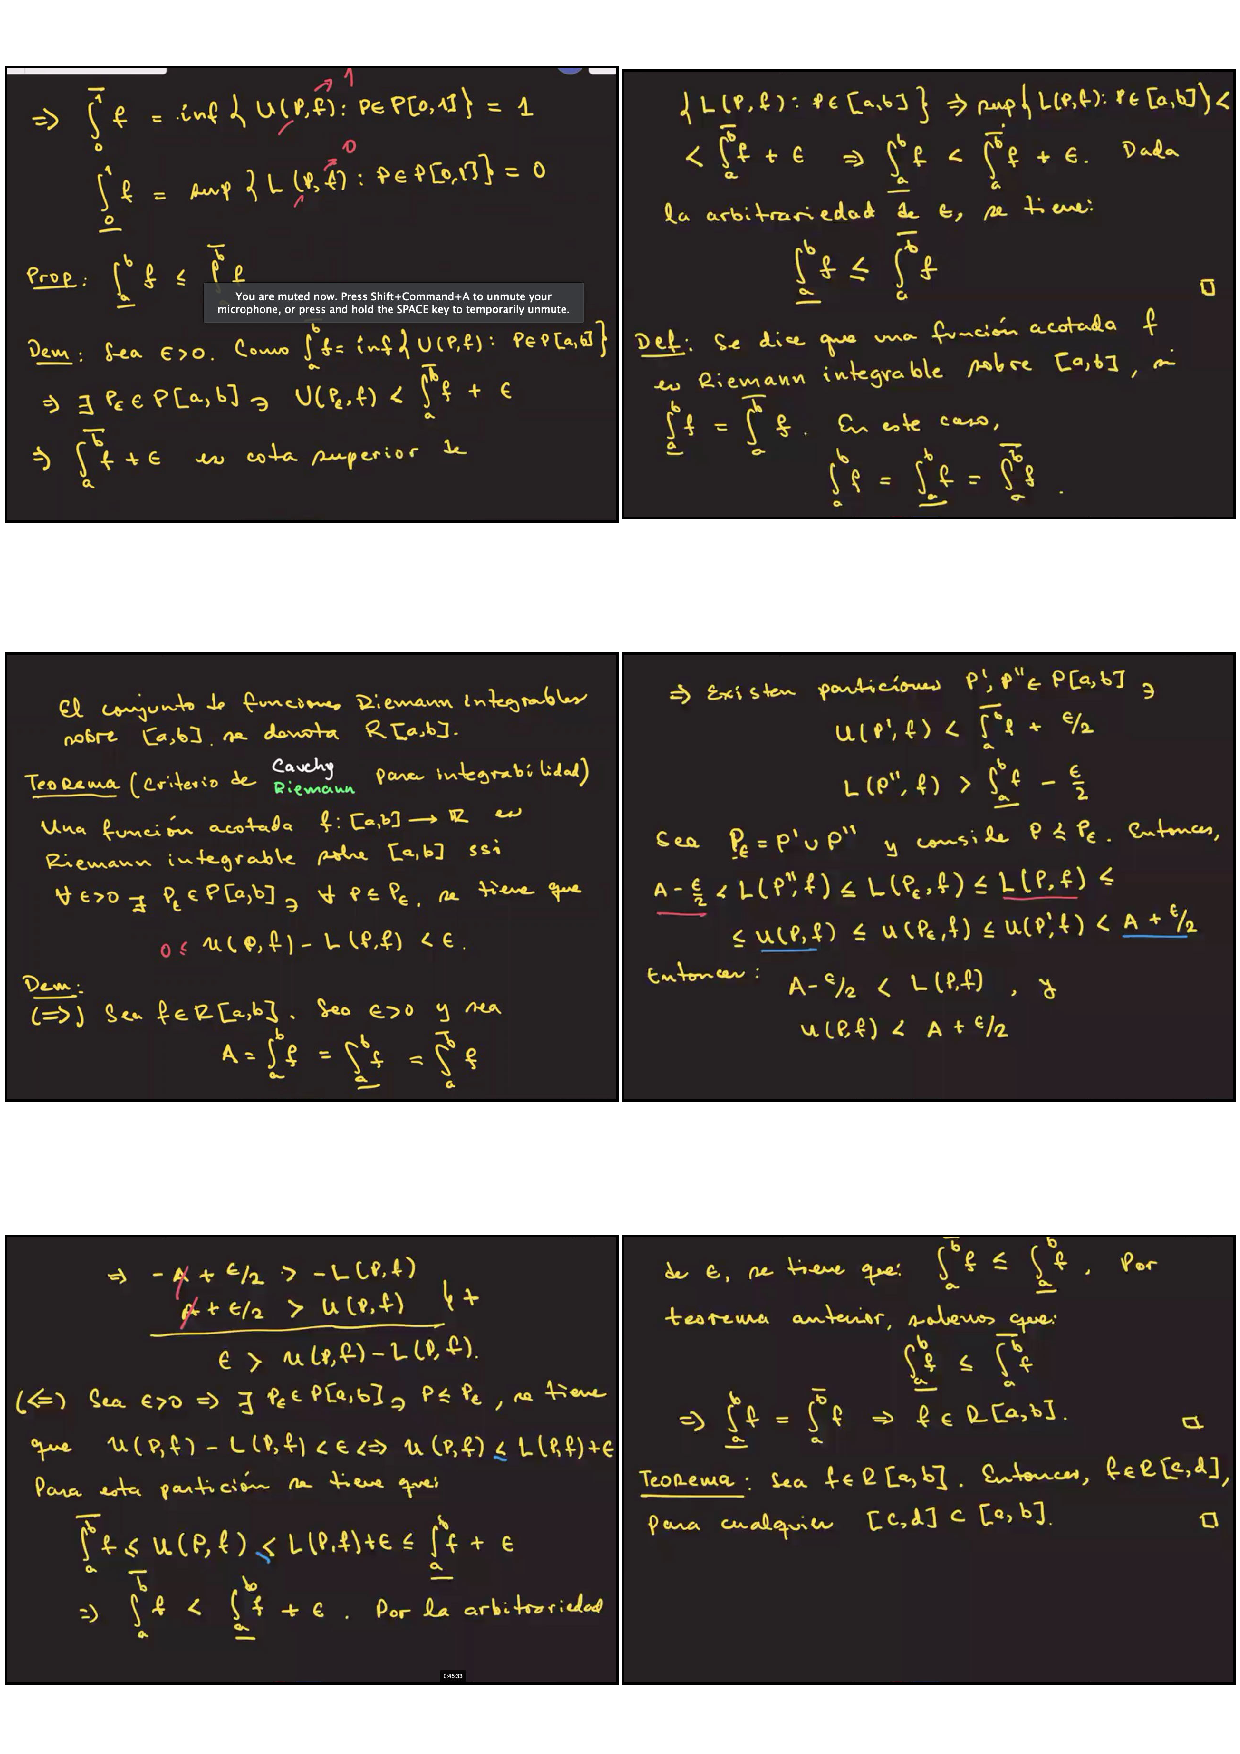
\includepdf[pages=-]{apendices/s2.pdf}